\let\negmedspace\undefined
\let\negthickspace\undefined
\documentclass[journal]{IEEEtran}
\usepackage[a5paper, margin=10mm, onecolumn]{geometry}
%\usepackage{lmodern} % Ensure lmodern is loaded for pdflatex
\usepackage{tfrupee} % Include tfrupee package

\setlength{\headheight}{1cm} % Set the height of the header box
\setlength{\headsep}{0mm}     % Set the distance between the header box and the top of the text

\usepackage{gvv-book}
\usepackage{gvv}
\usepackage{cite}
\usepackage{amsmath,amssymb,amsfonts,amsthm}
\usepackage{algorithmic}
\usepackage{graphicx}
\usepackage{textcomp}
\usepackage{xcolor}
\usepackage{txfonts}
\usepackage{listings}
\usepackage{enumitem}
\usepackage{mathtools}
\usepackage{gensymb}
\usepackage{comment}
\usepackage[breaklinks=true]{hyperref}
\usepackage{tkz-euclide} 
\usepackage{listings}
% \usepackage{gvv}                                        
\def\inputGnumericTable{}                                 
\usepackage[latin1]{inputenc}                                
\usepackage{color}                                            
\usepackage{array}                                            
\usepackage{longtable}                                       
\usepackage{calc}                                             
\usepackage{multirow}                                         
\usepackage{hhline}                                           
\usepackage{ifthen}                                           
\usepackage{lscape}
\begin{document}
\bibliographystyle{IEEEtran}
\vspace{3cm}

\title{5.2.62}
\author{EE25BTECH11060 - V.Namaswi}
% \maketitle
% \newpage
% \bigskip
{\let\newpage\relax\maketitle}
\renewcommand{\thefigure}{\theenumi}
\renewcommand{\thetable}{\theenumi}
\setlength{\intextsep}{10pt} % Space between text and floats
\textbf{Question}
Solve system of linear equations \\
\begin{align*}
3x-2y+3z=8\\2x+y-z=1\\4x-3y+2z=4
\end{align*}
\textbf{Solution}\\
According to question the Equations of line given are\\
\begin{align}
\begin{pmatrix}
  3 & -2 & 3  
\end{pmatrix}X=8\\
\begin{pmatrix}
   2 & 1 & -2  
\end{pmatrix}X=1\\
\begin{pmatrix}
 4 & -3 & 2   
\end{pmatrix}X=4\\
\begin{pmatrix}
    3 & -2 & 3 \\
    2 & 1 & -1\\
    4 & -3 & 2
\end{pmatrix}X=\begin{pmatrix}
    8 \\ 1\\ 4
\end{pmatrix}
\end{align} 
Forming Argumented Matrix\\
\begin{align}
\left(\begin{array}{ccc|c}
3 & -2 & 3 & 8 \\[4pt]
2 & 1 & -1 & 1 \\[4pt]
4 & -3 & 2 & 4
\end{array}\right).
\end{align}
Replace
 \[
R_1 \to \tfrac{1}{3}R_3
\]
\begin{align}
\augvec{3}{1}{
1 & -\frac{2}{3} & 1 &  \frac{8}{3} \\
2 & 1 & -1 & 1 \\
4 & -3 & 2 & 4}
\end{align}

Replace
\[
R_2 \to R_2 - 2R_1, 
\quad
R_3 \to R_3 - 4R_1
\]
\begin{align}
\augvec{3}{1}{
1 & -\tfrac{2}{3} & 1 & \tfrac{8}{3} \\
0 & \tfrac{7}{3} & -3 & -\tfrac{13}{3} \\
0 & -\tfrac{1}{3} & -2 & -\tfrac{20}{3}
        }
\end{align}
Replace
\[
R_2 \to \tfrac{3}{7}R_2
\]
\begin{align}
  \augvec{3}{1}{
1 & -\tfrac{2}{3} & 1 & \tfrac{8}{3} \\
0 & 1 & -\tfrac{9}{7} & -\tfrac{13}{7} \\
0 & -\tfrac{1}{3} & -2 & -\tfrac{20}{3}
 }  
\end{align}

Replace
\[
R_1 \to R_1 + \tfrac{2}{3}R_2, 
\quad
R_3 \to R_3 + \tfrac{1}{3}R_2
\]

\begin{align}
\augvec{3}{1}{ 
1 & 0 & \tfrac{5}{21} & \tfrac{22}{21} \\
0 & 1 & -\tfrac{9}{7} & -\tfrac{13}{7} \\
0 & 0 & -\tfrac{41}{21} & -\tfrac{143}{21}}
\end{align}
Replace
\[
R_3 \to -\tfrac{21}{41}R_3
\]
\begin{align}
\augvec{3}{1}{ 1 & 0 & \tfrac{5}{21} & \tfrac{22}{21} \\
0 & 1 & -\tfrac{9}{7} & -\tfrac{13}{7} \\ 
0 & 0 & 1 & \tfrac{143}{41} }
\end{align}

Replace
\[
R_1 \to R_1 - \tfrac{5}{21}R_3, 
\quad
R_2 \to R_2 + \tfrac{9}{7}R_3
\]
 \begin{align}
\augvec{3}{1}{1 & 0 & 0 & \tfrac{62}{123} \\
0 & 1 & 0 & \tfrac{110}{287} \\
0 & 0 & 1 & \tfrac{143}{41}}   
\end{align}
Hence,
 \begin{align}
\Vec{X}=\begin{pmatrix}
\tfrac{62}{123}\\ 
 \tfrac{110}{287} \\
 \tfrac{143}{41}
\end{pmatrix}
\end{align}
\centering
    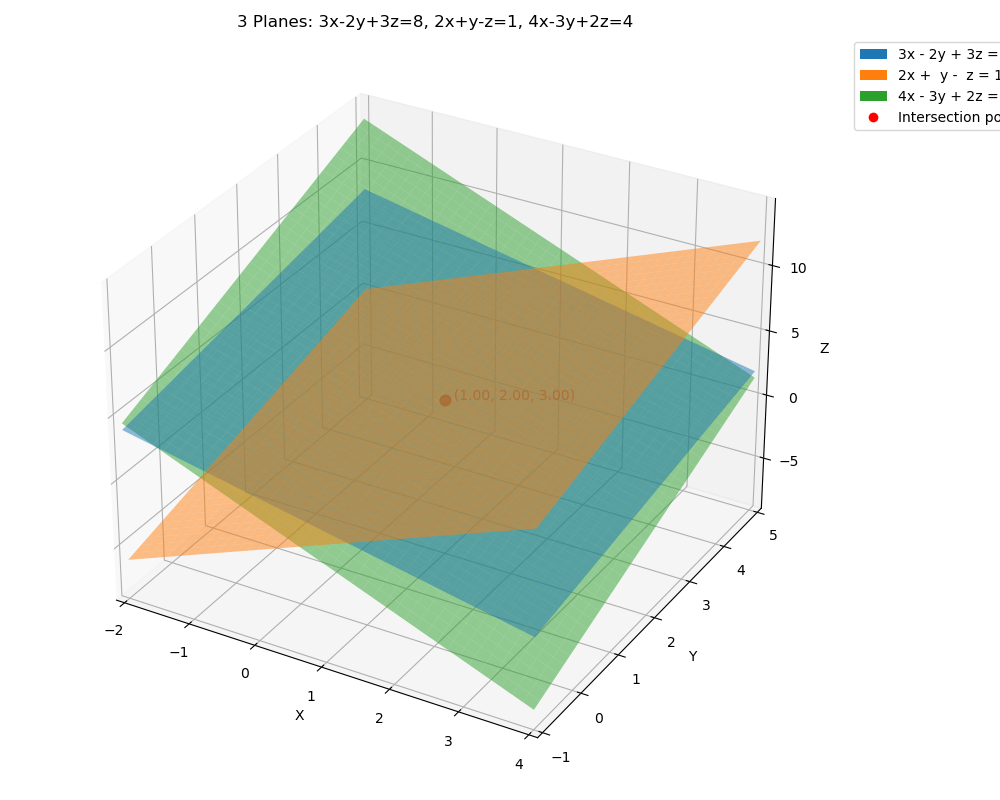
\includegraphics[width=\columnwidth, height=0.8\textheight, keepaspectratio]{fig/Figure_10.png}
\end{document}